\documentclass[11pt, a4paper]{article}

\usepackage[utf8]{inputenc}
\usepackage{authblk}
\usepackage{titlesec}


% Maths tools
\usepackage[tbtags]{amsmath}
\usepackage{amssymb}

% Margin
\usepackage[margin=2.9cm]{geometry}

% Line numbers
\usepackage{lineno}

% Spacing
\usepackage{setspace}
\doublespacing

% Enumeration
\usepackage{enumerate}% http://ctan.org/pkg/enumerate
\usepackage{enumitem}


% indentation
\setlength\parindent{10pt}
\setlength{\parskip}{5pt}

% Figures
\usepackage{graphicx}
\usepackage{caption}
\usepackage{subcaption}
\usepackage{epstopdf}
\usepackage{float}
\renewcommand{\thefigure}{\textbf{\arabic{figure}}}
\renewcommand{\figurename}{\textbf{Figure}}


%table
\usepackage{multirow}% http://ctan.org/pkg/multirow
\usepackage{hhline}
\usepackage[table]{xcolor}

\usepackage{authblk}


% References
\usepackage[round]{natbib}
\bibliographystyle{ecology_letters2.bst}

\usepackage{color, xcolor,soul}
%\definecolor{blau}{RGB}{168,221,181}
\definecolor{blau}{RGB}{236,226,240}
\soulregister\cite7
\soulregister\citenum7
\soulregister\citep7
\soulregister\citealt7
\soulregister\citealp7
\soulregister\citet7
\soulregister\ref7

% References and links
\PassOptionsToPackage{hyphens}{url}\usepackage[colorlinks=true,linkcolor=magenta, citecolor=magenta]{hyperref}

%Margin notes
\usepackage{marginnote}
% Foot note distance with text
\usepackage[symbol]{footmisc}
\renewcommand{\thefootnote}{\fnsymbol{footnote}}
\setlength{\skip\footins}{0.75cm}

%Define colour
\DeclareRobustCommand{\hlc}[1]{{\sethlcolor{blau}\hl{#1}}}

%subsubsection format
\titleformat*{\subsubsection}{\large\it}

\makeatletter
\renewcommand\AB@affilsepx{; \protect\Affilfont}
\makeatother

%Title paper
\title{\vspace{-1cm}
Model simplicity breeds contempt: using simple models to answer basic questions on species' distributions}
\author[1,*]{\normalsize Bernat Bramon Mora}
\author[1]{\normalsize Jake M.\ Alexander}
\affil[1]{\footnotesize Institute of Integrative Biology, ETH Zürich, Zürich, Switzerland}
\affil[*]{\footnotesize  bernat.bramon@gmail.com}

\renewcommand\Authands{ and }
\date{}

\begin{document}
\maketitle
\linenumbers

\section*{Abstract}
We know a lot about the factors that could theoretically influence species' distributions, and a rapidly growing body of research have been primarily focused on trying to untangle some of such biotic and abiotic predictors---with an increasing effort placed in improving the predictive power of statistical models. However, much less is known about how species' distributions compare to each other. Here, we use a conceptually more conservative approach to instead understand and compare basic aspects regarding the shape of species' distribution along environmental gradients.

\section*{Introduction}

%%%%%%%%%%%%%%%%%%%%%%%%%%%%%%%%
% PARAGRAPH 1
%%%%%%%%%%%%%%%%%%%%%%%%%%%%%%%%

One of the central goals of ecology is to understand the ways species are distributed across space (ref). Over the years, researchers have developed multiple distribution models to try to untangle the factors that play a role in defining such distributions (ref). These models estimate species' realized niches using several covariates, including environmental variables (ref), species ecological traits' (ref) and phylogenetic relations (ref). Moreover, recent work on these modelling approaches has focused on estimating (ref) and accounting for (ref) biotic factors, such as competitive or facilitative relationships. Overall, these methodological advances have provided with crucial ecological insights into the factors shaping species' distributions (ref); however, they have also faced some criticism as a result of the... For example, ...

The use of species distribution models has grown a lot. These models try to estimate species' realized niches using several covariates, including environmental variables (ref), species ecological traits' (ref) and phylogenetic relations (ref). Recent work on these modelling approaches has increasingly focused on estimating (ref) and accounting for (ref) biotic factors, such as competitive or facilitative relationships. The idea is that by understanding how all such factors shape species' distribution we will gain a mechanistic understanding on how these distributions are established and change over time. Unfortunately, while some of this approaches will certainly increase the predictive performance of distribution models (ref), the nature of some of the estimates have been shown to theoretically have some mishaps (ref).

%Ecology has been described as the scientific understanding of factors determining the abundance and distribution of species (Smith 1966; Begon et al. 1986). This understanding can hardly be achieved by studying species one by one since their abundances and distributions depend not only on their indi- vidual responses to the abiotic environment, but also on their interactions (Wisz et al. 2013). Thus, a key aim in modern community ecology is to gain an integrative understanding of how biotic and abiotic factors mould local species pools at different spatiotemporal scales. Community ecology began as a descriptive science in which communities were classified based on the identities and sizes of local species pools (e.g. Clements 1936; Elton 1966). Mod- ern community ecology is progressing from the description of patterns towards a mechanistic perspective, which seeks to understand the processes determining the identities and abundances of the species from local to global spatiotemporal scales (Agrawal et al. 2007; Logue et al. 2011). During the last few decades, experimental ecologist have used observations and experiments to assess the relative influences of stochastic- ity, competition and niche differentiation (see Logue et al. 2011), theoretical ecologists have developed models for pre- dicting community dynamics (e.g. Tilman 1990, 2004; Holt et al. 1994; Bolker et al. 2003; Leibold et al. 2004; Holyoak et al. 2005), and statistical ecologists have developed metrics for assessing compositional changes among local communities (e.g. Gauch 1982; ter Braak & Prentice 1988; Legendre & Legendre 2012).

%%%%%%%%%%%%%%%%%%%%%%%%%%%%%%%%
% PARAGRAPH 2
%%%%%%%%%%%%%%%%%%%%%%%%%%%%%%%%

Increasing efforts have been devoted to improving the ability of statistical models to predict the presence/absence of species across ranges (ref). Accurately predicting how species are distributed across ranges, it is crucial for understanding the impacts and effect of global climate change. With that said, accounting for the mechanisms can come at the cost of modelling noise... However, much less attention is paid to how species' distributions compare to each other. 


%\citet{austin2002spatial} writes "\textit{there are three major components in any framework for statistical modelling in plant ecology. There needs to be an ecological model, a data model, and a statistical model. The ecological model consists of the ecological knowledge and theory to be used or tested in the study. The data model consists of the decisions made regarding how the data are collected and how the data will be measured or estimated. The statistical model involves the choice of statistical method, error function and significance tests. Each model interacts in both obvious and subtle ways with the other models to determine the success of any statistical modelling exercise.}" While a lot of work has been developed for all three components outlined by \citet{austin2002spatial}, increasing emphasis has been put into advancing the data and statistical models. Indeed,

Increasing efforts have been devoted to improving the ability of statistical models to predict the presence/absence of species across ranges. However, much less attention is paid to how species' distributions compare to each other. 

%%%%%%%%%%%%%%%%%%%%%%%%%%%%%%%%
% PARAGRAPH 3
%%%%%%%%%%%%%%%%%%%%%%%%%%%%%%%%
A lot can be learned from the basic properties of species' realized niches.

Accounting for expert knowledge on species' environmental preferences to understand general distribution patterns.

%%%%%%%%%%%%%%%%%%%%%%%%%%%%%%%%
% PARAGRAPH 4
%%%%%%%%%%%%%%%%%%%%%%%%%%%%%%%%
Here, we...Bayesian framework... This allow us to account for... as well as to tackle long-standing hypothesis regarding basic aspects of species distributions. 


 
 
%%%%%%%%%%%%%%%%%%%%%%%%%%%%%%%%
% PARAGRAPH 5
%%%%%%%%%%%%%%%%%%%%%%%%%%%%%%%%
In this work, we first....

%%%%%%%%%%%%%%%%%%%%%%%%%%%%%%%%%%%%%%%
%%%%%%%%%%%   Stuff to realocate   %%%%%%%%%%%%%
%%%%%%%%%%%%%%%%%%%%%%%%%%%%%%%%%%%%%%%

There is no general agreement the shape of species distributions. While many ecological textbooks (Begon et al., 1990, Giller, 1984, Krebs, 1994) assume this to be unimodal and symmetric, some have warned that empirical distributions can take many different forms \citep{austin2002spatial}. There is not an easy way to untangle the true shape of species' distributions, as this shape is likely to showcase idiosyncrasies at the species level and across systems. The aim of this work, it is not to answer these questions nor to provide a general approach that accommodates such idiosyncrasies. Instead, we want to use a model that is solely constrained by the empirical information that we truly have regarding a particular system, relaxing as much as possible the structural constrains of the statistical framework. Then, we want to use this model to answer basic aspects regarding the way systems of many species are distributed along an environmental gradient. 

To decide among modelling approaches, we first needs to agree on what we know about the system. We know that species occupy a geographic range; therefore, we know that their distributions have finite variance. Indeed, observations on species' geographic variation and optimal climatic conditions have been long documented, with extensive databases compiled by botanists and field ecologists documenting basic knowledge on species' distributions. One could point out that we also know that many other factors might influence species' presence/absence---e.g. the influence of biotic interactions among species. However, we do not necessarily have an intuition of how exactly these factors will influence the shape of species' distributions. As a result, if all we truly knew about a species' distribution was that they have finite variance, the most conservative assumption and the safest bet---i.e. the one with the largest entropy---is that such distribution is a Gaussian.

%There is a growing literature on species' distribution models. For the most part, however, these models have often focussed on model performance and understanding the predictive power of certain covariates. This models often take a response variable, such as presence/absence or abundance data, and fit it with a set of environmental variables and species' ecological or phylogenetic relationships. There... The shape of distributions on systems of many species is rarely studied. That is, simple ...
%model comparison... 
%creating maps of relative suitabilities...
%extrapolate to new data...

%It will be argued in this paper that neglect of ecological knowledge is a limiting factor in the application of statistical modelling in ecology and conservation planning

%The field has shifted towards understanding the effects of biotic factors on such distributions. And while the theory is advancing quickly, the...

%This is a generalised additive model.
% Results are presented for both simulated and empirical data.
% But this approach understates the posterior uncertainty in inference. 
%\section*{Introduction}

%%%%%%%%%%%%%%%%%%%%%%%
% Paragraph on Rapoport's rule
%%%%%%%%%%%%%%%%%%%%%%%
% McCain
%Understanding the factors that determine species range size dis- tributions is becoming increasingly urgent as more climate change assessments document the heightened risk for small- ranged species (e.g. Channell & Lomolino, 2000; Sekercioglu et al., 2008; La Sorte & Jetz, 2010; McCain & Colwell, 2011).
%Rapoport’s rule is the positive relationship of species range sizes with increasing latitude (Stevens, 1989), elevation (Stevens, 1992) or water depth (Stevens, 1996). The latitudinal Rapoport’s rule (LRR) is the most examined in the literature, including testing empirical datasets (e.g. Rohde et al., 1993; Roy et al., 1994; Blackburn & Gaston, 1996; Lyons & Willig, 1997; Ruggiero & Lawton, 1998; Reed, 2003; Arita et al., 2005; Hausdorf, 2006), simulation modelling of the expected patterns (Colwell & Hurtt, 1994; Taylor & Gaines, 1999; Case & Taper, 2000; Arita, 2005; Stauffer & Rohde, 2006; Šizling et al., 2009), and theoretical and empirical evidence for the proposed mechanisms (e.g. Rohde, 1992; Kerr, 1999; Taylor & Gaines, 1999; Gaston & Chown, 1999a; Addo-Bediako et al., 2000; Parmesan et al., 2005). The various reviews of the LRR to date suggest that the overall support is weak (e.g. Rohde, 1996; Gaston et al., 1998; Rohde, 1999; Gaston & Chown, 1999b; Ribas & Schoereder, 2006), prin- cipally due to the high degree of variability in the fit to predic- tions (e.g. support: Blackburn & Gaston, 1996; Lyons & Willig, 1997; Price et al., 1997; Arita et al., 2005; no support: Rohde et al., 1993; Roy et al., 1994; Ruggiero & Lawton, 1998; Reed, 2003).
%The elevational Rapoport’s rule (ERR) has received less examination in the literature than the LRR, but there have also been empirical tests of its predictions (e.g. Patterson et al., 1996; Pleguezuelos & Villafranca, 1997; Price et al., 1997; Rahbek, 1997; Fleishman et al., 1998; Ruggiero & Lawton, 1998; Nathan & Werner, 1999; Sanders, 2002; Fu et al., 2004; Chatzaki et al., 2005; Almeida-Neto et al., 2006; Bhattarai & Vetaas, 2006; Hausdorf, 2006) and underlying theory (e.g. Rohde, 1996; Fleishman et al., 1998; Gaston & Chown, 1999a; Hausdorf, 2006; Ribas & Schoereder, 2006). In the ERR, like the LRR, there is a high degree of variability in support from supportive (e.g. Pat- terson et al., 1996; Pleguezuelos & Villafranca, 1997; Price et al., 1997; Rahbek, 1997; Fleishman et al., 1998; Sanders, 2002; Chatzaki et al., 2005; Almeida-Neto et al., 2006; Hausdorf, 2006; Ribas & Schoereder, 2006) to little or no support (e.g. Patterson et al., 1996; Price et al., 1997; Rahbek, 1997; Ruggiero & Lawton, 1998; Nathan & Werner, 1999; Fu et al., 2004; Bhattarai & Vetaas, 2006; Hausdorf, 2006; Ribas & Schoereder, 2006). Similarly, the processes proposed to underlie the ERR (Stevens, 1992) also show a variable amount of theoretical and empirical support (Patterson et al., 1996; Rohde, 1996; Rahbek, 1997; Fleishman et al., 1998; Gaston & Chown, 1999a; Almeida-Neto et al., 2006; Hausdorf, 2006; Colwell, 2011).
Scarce data and little to no attempt to account for uncertainty in the predictions. Similar to rapoport's rule, we can also ask other questions regarding general geographical patterns of species distributions. 

\section*{Methods}
\subsection*{Empirical data}
We studied the distribution of alpine plant communities along an elevation gradient. To do so, we combined two different datasets: i) one describing the co-occurrence of species across multiple open grasslands in the Swiss Alps, and ii) an extensive floristic database containing environmental and physiological traits for all vegetation across Switzerland \citep{landoltFloraIndicativaOkologische2010}. 

\subsubsection*{Distribution data}
We studied the distribution of 798 species across 912 sites covering most of the mountain region of the Western Alps in the Canton de Vaud (Switzerland; \citealt{scherrerEcologicalIndicatorValues2019}). Each of these sites is a $8\times 8\,\text{m}$ plot placed somewhere along an elevation range from $375\,\text{m}$ to $3210\,\text{m}$. In all sites, presence/absence data as well as Braun-Blanquet abundance-dominance classes were recorded for all species. Additionally, following 30 years (1961–1990) of meteorological data from national weather stations, \citet{scherrerEcologicalIndicatorValues2019} calculated multiple climatic variables for each site at high spatial resolution ($25\,\text{m}$). Here, we focussed on 9 climatic variables, including: daily minimum, maximum and average temperature; sum of growing degree-days above $5^{\circ}\text{C}$; mean temperature of wettest quarter; annual precipitation, precipitation seasonality, and precipitation of driest quarter. %Missing TabsY

\subsubsection*{Floristic data}
To complement the aforementioned distribution data, we used a floristic database of most vegetation across Switzerland. This database was build based on expert knowledge and field experience of botanists and ecologists, and contains information regarding species' environmental preferences and physiological traits. Species' environmental preferences in this database can be used to inform distribution models---e.g. as an informative prior in a Bayesian framework. These are characterized following the ecological indicator values developed by \citet{landoltFloraIndicativaOkologische2010}, providing both an estimate of the average conditions in which a species can be found and a broad description of their range of variation. These values are provided for a range of 10 climatic variables, including temperature, continentality, light conditions, as well as moisture, acidity and nutrient content of the soil (see a full list and description of the ecological indicators in the Supplementary Methods; \citealt{landoltFloraIndicativaOkologische2010}). On the other hand, the information regarding species' physiological traits represent general descriptions of species' growth and life strategies---examples include their growth forms, nature of the storage organs, dispersal ability and pollinator agents. In total, we identify more than $120$ binary traits that characterize the physiology of species (see a full list and description of the ecological indicators in the Supplementary Methods; \citealt{landoltFloraIndicativaOkologische2010}).  

%we independently consider those traits that describe growth and life strategies of the plants---examples include their growth forms, nature of the storage organs, dispersal ability and pollinator agents. In total, we identify $\sim120$ binary traits that characterize the physiology of species.

%comprising a total of 10 environmental indicator values with 10 types of associations for each of them (i.e. the $r$ associations defined above). Finally, we additionally independently consider species' range of variations for the such indicator values, also defining 10 `traits' with 3 types of associations (I need to see if I can added these to the analyses above).

%In this study we used the ecological indicator values (EIVs) first developed by Landolt17 and later extended by Landolt et al.19. Landolt’s EIVs are largely similar to the more renown ones proposed by Ellenberg et al.18, but specifically adapted to the flora and environmental conditions of Switzerland. There are a large number of EIVs (for details see Landolt et al.19), but in this study we focused on six of the most commonly used, namely: T for temperature;, M for soil moisture/water availability;, L for light;, K for continentality;, R for soil pH; and N for soil nutrients.
%Based on 30 years (1961–1990) of meteorological data from national weather stations, fourteen climatic variables (Table S5) were calculated according to the method described in Zimmermann & Kienast44 and Zimmerman et al.55. A digital elevation model (DEM) was used to spatially interpolate the climatic data and to create topographic variables (Table S5). Additionally, we used a soil pH map based on Buri et al.43. All environmental data had a spatial resolution of 25 m, a resolution similar to the areas used to calculate the ecological indicator values (EIV; see below). This allowed a straightforward comparison of different sets of predictors composed from environmental variables and EIVs.

%In this study we used the ecological indicator values (EIVs) first developed by Landolt17 and later extended by Landolt et al.19. Landolt’s EIVs are largely similar to the more renown ones proposed by Ellenberg et al.18, but specifically adapted to the flora and environmental conditions of Switzerland. There are a large number of EIVs (for details see Landolt et al.19), but in this study we focused on six of the most commonly used, namely: T for temperature;, M for soil moisture/water availability;, L for light;, K for continentality;, R for soil pH; and N for soil nutrients.

{\color{gray}
\subsubsection*{[Trait data]}
This could be Tom's data if we end up using it.}

\subsection*{Distribution model}
There is a long list of model structures well suited to characterize species' distributions (see XX for a review); however, we were interested in a model that explicitly incorporates all information regarding plant's environmental preferences found in the floristic database. More specifically, we wanted to account for the climatic indicator values and range of variation registered for all plants in our dataset. These two values provide basic information regarding plant's optimal environmental conditions and width of their distributions. Therefore, we first formulated a baseline model that directly accounts for such prior information. 

\subsubsection*{Baseline model}
Given $y_{ij}$ the presence/absence of any species $i$ in any given site $j$, and a set of $k$ environmental variables $x_{jk}$, we estimate species' distributions as:
\begin{equation} 
\begin{split}
y_{ij} & \sim \text{Binomial}\left(1, p_{ij}\right)\\
\text{log}\left(p_{ij}\right) & = -\alpha_{i} - \sum_{k} \lambda_{ik} \left(x_{jk}-\beta_{ik}\right)^2\\
\text{log}(\alpha)  & \sim \text{MVNormal}\Big(\hat{\alpha}, \Sigma^{\alpha}\Big)\\
\beta_{ik}  & \sim \text{MVNormal}\left(\hat{\beta}_{k}, \Sigma^{\beta_{k}}\right)\\
\text{log}(\lambda_{ik})  & \sim \text{MVNormal}\left(\hat{\lambda_{k}}, \Sigma^{\lambda_{k}}\right)\\
\hat{\alpha}, 
\hat{\lambda^{k}}, 
\hat{\beta^{k}}  & \sim \text{Normal}\left(0,1\right)
\end{split}
\label{eq:baseline}
\end{equation}
Notice that this model structure assumes all plants to have a uni-modal distributions along each environmental axis (see the model's behaviour in Supplementary Figure XX), where parameters $\alpha_i$, $\beta_i^k$, and $\lambda_i^k$ describe amplitude of the probability $p_{ij}$, species' average climatic suitability and range of variation along the different environmental gradients, respectively\footnote[2]{I'll rewrite the likelihood function to an ordered categorical as soon as I get things to work properly with count data.}. While potentially sacrificing predictive accuracy, this model structure allows us to explicitly incorporate all prior knowledge that we have regarding species' distributions via $\Sigma^{\alpha}$, $\Sigma^{\beta_{k}}$ and $\Sigma^{\lambda_{k}}$. More specifically, we express $\beta_i^k$ and $\log\left(\lambda_i^k\right)$ as multivariate normal distributions---i.e. Gaussian processes---such that $\Sigma^{\beta_{k}}$ and $\Sigma^{\lambda_{k}}$ are variance-covariance matrices describing species' similarity in terms of their average climatic suitability and range of variation along the different environmental gradients, respectively. Likewise, $\log\left(\alpha\right)$ is characterized as a Gaussian Process, where the corresponding variance-covariance matrix $\Sigma^{\alpha}$ is designed to also incorporate some of the prior information that we have with regards to species' physiological traits.

In all cases, all variance-covariance matrices are defined as follows:
\begin{equation} 
\Sigma^{\chi}_{ij} = \eta_{\chi}\,\text{exp}\left(-\rho_{\chi} {D^{\chi}_{ij}}^2\right) + \delta_{ij} \sigma_{\chi} ,
\label{eq:covariance}
\end{equation}

where $\Sigma^{\chi}_{ij}$ describes the covariance between any pair of species $i$ and $j$ for any given parameter $\alpha_i$, $\beta_i^k$, and $\lambda_i^k$. Following this expression, such covariance declines exponentially with the square of the different $D^{\chi}_{ij}$, which are distance measures computed using the prior information that we have regarding species' distributions. Specifically, given $\alpha_i$, $\beta_i^k$, and $\lambda_i^k$, the distance measures are calculated using plants' physiological traits, ecological indicator values and range of variation, respectively (see below for further details). For each covariance matrix, the hyperparameter $\rho_{\chi}$ determines the rate of decline of the covariance between any two species, and $\eta_{\chi}$ defines its maximum value. The hyperparameter $\sigma_{\chi}$ describes the additional covariance between the different observations for any given species. For any given hyperparameter, we choose adaptive priors across covariance structures. That is, and taking $\rho_{\chi}$ as an example, we choose a prior $\log\left(\rho_{\chi}\right)\sim \text{Normal}\left(\hat{\rho}, \sigma_{\rho}\right)$ such that $\hat{\rho}\sim \text{Normal}\left(0, 1\right)$ and $\sigma_{\rho}\sim \text{Exponential}\left(1\right)$. Similar priors were chosen for both $\eta_{\chi}$ and $\sigma_{\chi}$. We generated the posterior samples for the Bayesian models with the help of the R package `rstan' to \citep{rstan}.

\subsubsection*{Distance matrices}
The missing component in the description of model (\ref{eq:baseline}) is the distance matrices $D^{\chi}$ used to define the covariance matrices $\Sigma^{\alpha}$, $\Sigma^{\beta_{k}}$ and $\Sigma^{\lambda_{k}}$. In this model, such distance matrices characterize differences between plant species. In the floristic data, however, the prior information that we have for these differences is represented by a set of ordinal and categorical traits. More specifically, both the ecological indicator values and range of variation---which define the prior information that we have for $\beta_i^k$, and $\lambda_i^k$, respectively---are ordinal traits specified for all species. In contrast, the plants' physiological data---shaping the prior for the parameters $\alpha_i$---are characterized by categorical data containing multiple missing entries. Therefore, we need to carefully compile this data into distance matrices in order to be able to feed this prior information into the model. 

More generally, we want to understand the way $N$ species are characterized by $M$ categorical traits. One way to frame this problem is by using a network representation. Following the ideas presented by \citet{godoy-loriteAccurateScalableSocial2016}, we assume that species can be connected to each of these traits by an interaction $\left(i, j\right)$ that can be of any type $r\in R$. Notice that this provides as with multiple ways to account for the information---and lack thereof---contained in the different categorical and ordinal traits $M$. That is, the $R$ types of interactions can represent the lack of information for a particular link $\left(i, j\right)$, the absence or presence of such interaction, and any type of association between $i$ and $j$. 

Given a set of interactions $R^{*}$ between $N$ and $M$, we use a Mixed Membership Stochastic Block Model (MMSBM) to characterize these. In particular, we consider that plants and traits can be classified into $K$ and $L$ groups, respectively. For every species $i$, we assume that there is a probability $\theta_{i\alpha}$ for it to belong to any of the $K$ species groups. Likewise, we also assume that any trait $j$ has a probability $\phi_{j\beta}$ of belonging to any of the $L$ trait groups. Finally, we define $p_{\alpha\beta}\left(r\right)$ as the probability of a species from group $\alpha$ interacting with a trait from group $\beta$ by an association type $r$. Putting these together, the probability of an interaction $\left(i, j\right)$ of type $r$ can be calculated as:
\begin{equation}
Pr[r_{ij}=r] = \sum_{\alpha \beta} \theta_{i\alpha} \phi_{j\beta} p_{\alpha\beta}\left(r\right)
\end{equation}
Following this definition, we want to find the group memberships that maximize the likelihood $P\left(R^{*}|\theta, \phi, p\right)$. Doing so is difficult optimization problem; however, it has been shown that one can estimate the different $\theta_{i\alpha}$, $\phi_{j\beta}$, and $p_{\alpha\beta}\left(r\right)$ parameters by maximizing the likelihood using an expectation-maximization algorithm \citep{godoy-loriteAccurateScalableSocial2016, tarres-deulofeuTensorialBipartiteBlock2019}. In simple terms, one can iteratively find multiple local minima for the likelihood, and average over the estimated the parameter values \citep{godoy-loriteAccurateScalableSocial2016}\footnote[2]{
While this averaging is trivial for the estimated probabilities $Pr[r_{ij}=r]$, it is non-trivial if one wants to find averages for the group memberships. The reason for this is related to the stochastic nature of the expectation-maximization algorithm. This algorithm initially assigns random group memberships to both species and traits. While this random labelling is irrelevant when studying the probabilities $Pr[r_{ij}=r]$, it is instead crucial for averaging $\theta_{i\alpha}$, $\phi_{j\beta}$, and $p_{\alpha\beta}\left(r\right)$. Therefore, before averaging the group membership estimates, one needs to find the bijective relationship for the labellings of different iterations of the optimization algorithm. In a nutshell, for every iteration, I do this by using a simulated annealing algorithm on the estimated $p_{\alpha\beta}\left(r\right)$, matching the corresponding labelling to a reference iteration.}. 

The average estimates for the group memberships provide us with a different scale to classify species based on the traits these have. In short, for any species $i$, we can estimate a $K$-dimensional vector $\vec{\theta}_{i}$ that describes the extend to which $i$ belong to each group membership---i.e. the extend to which a species is of one type or another. This classification is useful because it can be used to compare species, defining a way to measure the distance between species based on an arbitrary---and potentially incomplete---set of categorical or ordinal traits $M$. The simplest case is to define the distance as $D_{ij} = |\vec{\theta}_{i}-\vec{\theta}_{j}|$. Alternatively, one could also define $K$ distance matrices based on the different group memberships $D^{\alpha}_{ij} = |\theta_{i\alpha}-\theta_{j\alpha}|$.

\subsubsection*{Modifying the variance-covariance structures}
The model structure defined in Eq.~(\ref{eq:baseline}) allows us to test the effect of adding new information. Specifically, we can do this by modifying Eq.~(\ref{eq:covariance}). For example, imagine that we have multiple matrices $D^k$ characterizing species' differences along different axis of variation---i.e. two matrices characterizing ecological and environmental traits, or multiple matrices resulting from the different group memberships estimated using the MMSBM. One could modify Eq.~(\ref{eq:covariance}) for a particular parameter---e.g. parameter $\alpha_i$---such that
\begin{equation} 
\Sigma^{\alpha}_{ij} = \eta_{\alpha}\,\text{exp}\left(-\sum_k\rho_{\alpha k} {D^{k}_{ij}}^2\right) + \delta_{ij} \sigma_{\alpha} ,
\label{eq:covariance-complex}
\end{equation}
where now $\rho_{\alpha k}$ are separate relevance hyperparameters for each distance matrix in the total variance of $\alpha_i$. Notice that the same is true for the covariance of parameters $\beta_i^k$ and $\lambda_i^k$. Finally, for all hyperparameters and as described for the baseline model, we use adaptive priors across covariance structures.

\section*{Results}
%We first use the baseline model to estimate the distribution of all species with at least 10 occurrences using all the data that we have with regard to...
\begin{figure}[ht]
  \centering
    \vspace{0.5cm}
    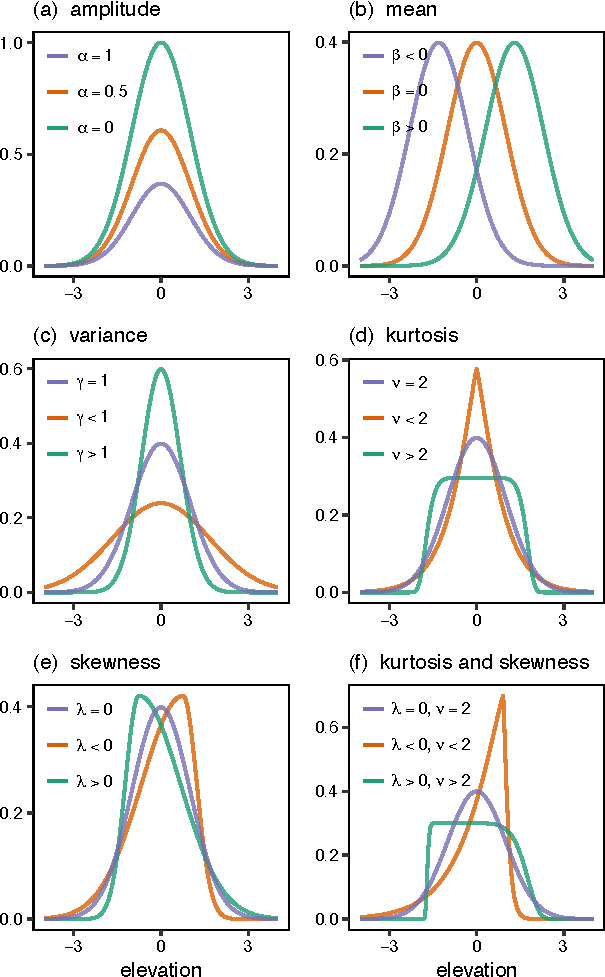
\includegraphics[width=0.9\textwidth]{figures/figure1}
    	  \vspace{0.3cm}
	   \caption{Relationship between mean and variance of species' distributions. These are the results for the main axis of variation for the climatic data (results for the second axis of variation presented in the Supplementary Fig.~2).}
      \label{fig:correlation}
\end{figure}

\begin{figure}[h]
  \centering
    \vspace{0.5cm}
    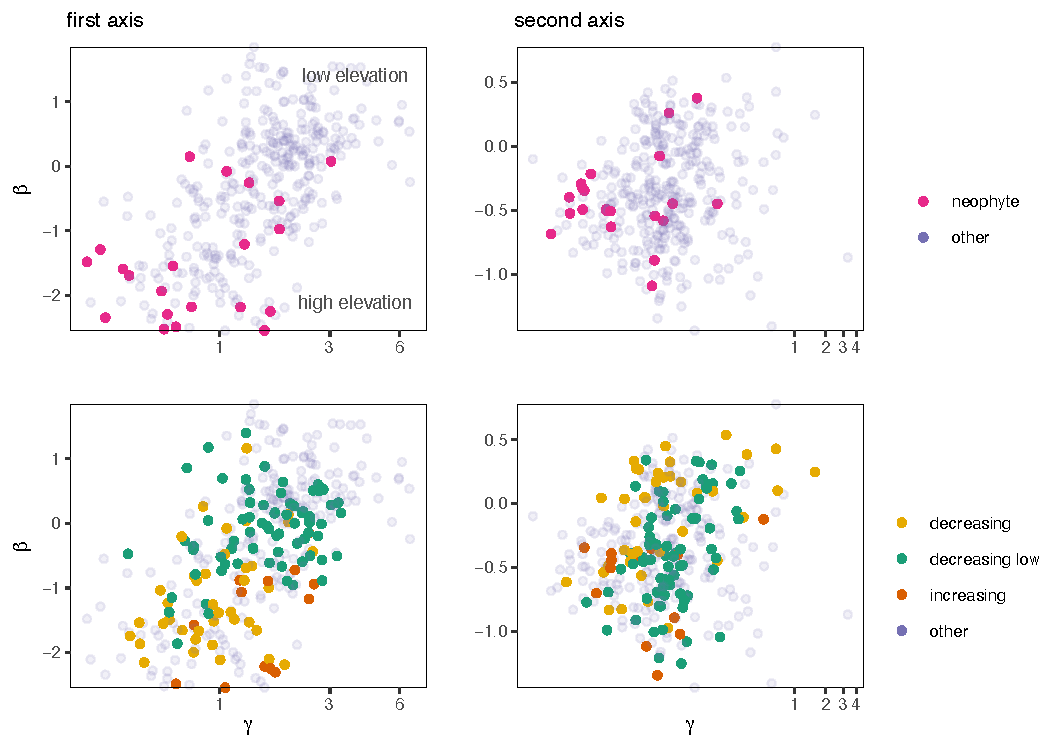
\includegraphics[width=0.9\textwidth]{figures/invasive}
    	  \vspace{0.3cm}
	   \caption{Are there clear geographical patterns for neophytes and for species with decreasing or increasing abundance?}
      \label{fig:neophytes}
\end{figure}

%\section*{Discussion}
\clearpage
\bibliography{references}

\end{document}
